\section{Concepts and approach}

Several deep learning techniques are required in order to achieve the final goal of the project. Tasks like feature extraction from Atari frames, generation of latent space representation and finding and training of the agent's policy will require different types of neural networks.

When dealing with Atari games, the problem of constructing features vectors from raw pixels can be addressed using \textbf{convolutional neural networks (CNNs)}.
CNNs are a class of neural networks designed to process ``grid-like topology data'' (\cite{goodfellow2016deep}) like images or audio signals. CNNs allow to ``abstract'' features from raw pixel matrices using an operation called \textit{convolution}, a special kind of linear operation. Each feature will be represented by a \textit{filter}: a vector of weights and a respective bias that are incrementally adjusted to ``learn'' how to correctly extract that specific feature (e.g. a square shape). 
Furthermore, by using gameplay frames as input for the CNN, we assure that each task that is later embedded in the latent space has the same data structure for the state space.  

In order to generate a latent space representation, \textbf{autoencoders} will be used. An autoencoder is a neural network consisting of two parts: the encoder, which converts the input to a dense and smaller representation and the decoder, which rebuilds the input from the compressed representation. The main application for autoencoders is dimensionality reduction (\cite{Hinton504}), where the encoder learns to preserve meaningful attributes of the input and generates a lower dimensional representation that is saved in the \textbf{latent space}. 

In this case, we intend to use the latent space as a generalized representation of the state spaces of different but related reinforcement learning tasks. To create a continuous latent space, that could allow transfer among tasks, a \textbf{variational autoencoder (VAE)} will be used. This kind of neural network uses probability distributions to describe each feature, allowing interpolation and random sampling in the data. Moreover, VAEs are trained with \textbf{gradient based methods} which give a better control over the latent space representation (\cite{goodfellow2016deep}) and can be used to generate representations with disentangled factors (\cite{2016arXiv160605579H}).

To achieve transfer learning, the agent will learn from the shared latent representation. 
% using deep reinforcement learning techniques. This algorithms will be used with the objective of creating an agent that will be capable of detecting similar states and situations that occur on tasks and act in a similar way in each of them. 
Two approaches of reinforcement learning will be taken into consideration. On the one hand, \textbf{deep Q-learning (DQN)} makes use of a special type of neural network called deep Q-network which is used to approximate the reward based on the state, called Q-value. The objective of this method is to find a function that maximize that value, which is the expected reward after taking a specific action in a certain  state. On the other hand, \textbf{policy gradients} follow a simpler approach and try to learn the policy function that maps the state to the action directly. This method learns from past trajectories, increasing the probability of actions which in the past returned good results for the agent.

Figure \ref{framework} briefly illustrates the the approach described above. From the VAE shown on the left hand side, we seek to derive a shared latent representation of several source tasks. We are interested in whether a target task could also be represented in this latent state and benefit from previously learned knowledge on the source tasks, as shown on the right hand side of the figure.

\begin{figure}[h!]
	\centering
	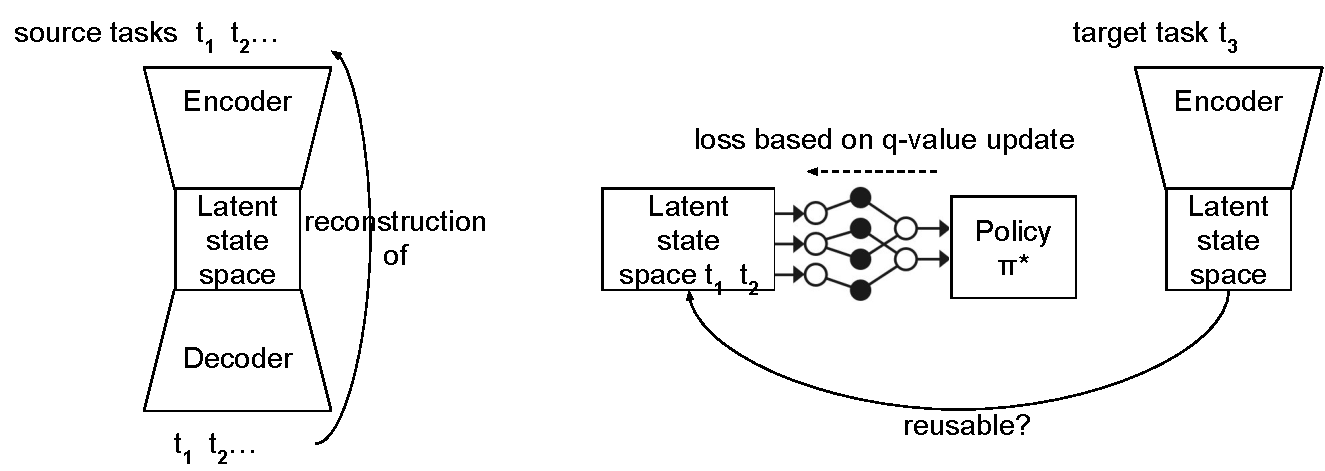
\includegraphics[width=\textwidth,height=\textheight,keepaspectratio]{framework.pdf}
	\caption{An illustration of transfer learning framework.}
	\label{framework}
\end{figure}


% Concepts:
% \begin{itemize}
% \item Existing Technologies
% \item Methods
% \item Terminology
% \end{itemize}

% Approach:
% \begin{itemize}
% \item What will you be doing with these technologies?
% \item How will you apply them?
% \end{itemize}